\chapter{Estado del Arte}
\label{sec:EstadoDelArte}
La estimación de calidad de imágenes y objetos 3D, al ser un componente sumamente 
ligado al avance tecnológico y necesidades de manejo de información digital, ha 
tomado mayor interés en el comienzo del siglo actual.
Puede observarse en la Figura \ref{fig:ScopusMLinMedicalAndPC} que existe 
una tendencia creciente en el número de publicaciones en relación a la aplicación 
de inteligencia artificial en las nubes de puntos y en imágenes médicas, llegando
ambas a sobrepasar 6000 documentos a partir de 2020.  Vemos que ambos incluso siguen 
lado al lado en número de publicaciones cuando especificamos que sean documentos 
relacionados con la estimación de calidad, sobrepasando los 250 documentos. 
Por otro lado, y afirmando lo mencionado sobre el bajo número de publicaciones 
en el ámbito biomédico para la estimación de calidad en 3D, vemos que, aunque hay
también una tendencia positiva, en 2022 tenemos solo 62 publicaciones. Esto 
se interpreta como indicador de lo novedoso y pionero de este proyecto.
\footnotetext[1]{
  Las búsquedas se pueden consultar en el Apéndice \ref{subs:Scopus}
}
\begin{figure}[H]
  \centering
  \begin{subfigure}{0.49\textwidth}
    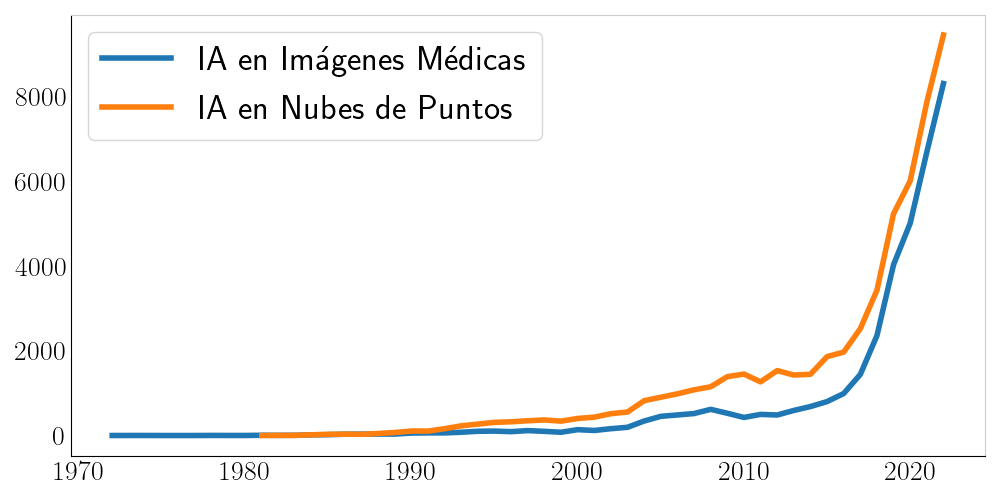
\includegraphics[width=\textwidth]{imagenes/chapter3/ScopusMLinMedicineAndPC.png}
  \end{subfigure}
  \begin{subfigure}{0.5\textwidth}
    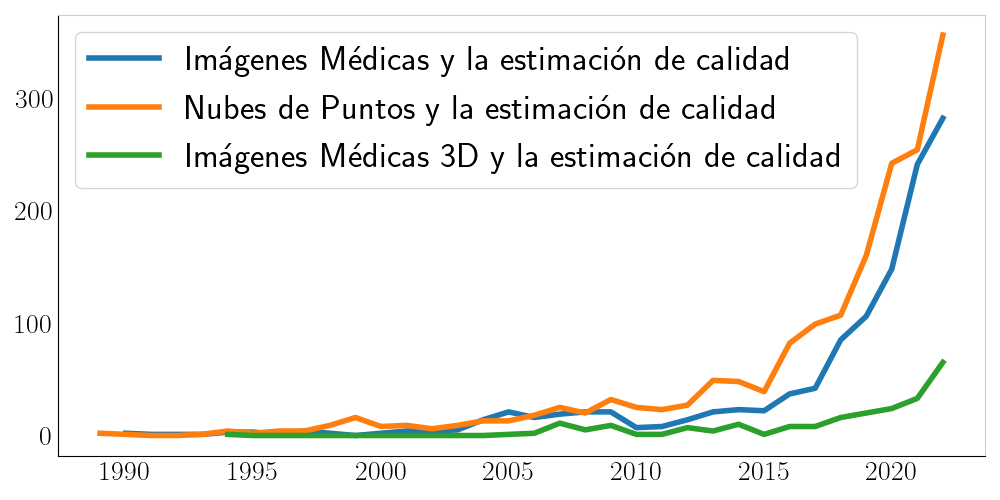
\includegraphics[width=\textwidth]{imagenes/chapter3/ScopusQualityAssessment.png}
  \end{subfigure}
  \caption[Crecimiento de interés en el campo según \emph{Scopus}]{Crecimiento de interés en el campo según \emph{Scopus}\footnotemark[1].
  A la izquierda podemos ver un incremento de publicaciones desde 
  1970 sobre la IA aplicada a nubes de punto, en naranja, 
  y aplicada de forma general a imágenes médicas, en azul. A la derecha 
  podemos ver de forma similar el crecimiento de métodos aplicados
  a la estimación de calidad a nubes de puntos, naranja, a imágenes médicas, azul, y 
  a imágenes médicas 3D, verde.
  }
  \label{fig:ScopusMLinMedicalAndPC}
\end{figure}

\section{Estado del arte de IQA}
Para la resolución del problema, tanto FR como NR, ha sido crucial los avances de los conocimientos 
del sistema visual humano. Se han propuesto métricas inspiradas en el HVS y 
conscientes del contenido de la imagen, que combinan las características del HVS 
con algoritmos matemáticos. En FR por ejemplo, Visual SNR\cite{VSNR} cuantifica 
la fidelidad visual de las imágenes con el ratio de relación entre señal-ruido y 
PSNR-HVS\cite{PSNR-HVS} combina el ese ratio con la función que determina 
nuestra sensibilidad al contraste. 
Wang y Bovik afirmaron que los ojos humanos obtienen información de imagen a 
través de tres canales: brillo, contraste y estructura\cite{SSIM} y desarrollaron 
un índice universal de calidad de imagen (UQI, por sus siglas en inglés) \cite{UQI} y una similitud 
estructural (SSIM)\cite{SSIM} para problemas FR. Surgieron incluso métodos que, basados en las 
respuestas del HVS, introducen la saliencia visual\footnote{
  Cualidad estética de la forma de un objeto o una configuración que destaca.
}en la evaluación de la calidad de imagen (por ejemplo, VSI)\cite{VSI}, 
ya que se ha observado que la saliencia de la imagen desempeña un papel importante.

Desde entonces se han propuesto diversas variantes de estos métodos, adaptadas 
al contexto y información disponible. 
Para la estimación de calidad de las imágenes sin referencia surgieron métricas para 
tipos de distorsiones específicas como 
imágenes borrosas\cite{GradientBasedBlurAssessment}, 
imágenes comprimidas en JPEG\cite{JPEGBasedOnLuminance}, 
imágenes con artefactos de bloque\cite{DeblockedImages} y imágenes con 
cambios de contraste\cite{ContrastDistorted}.
Luego, se buscaron maneras de estimar la calidad de imágenes de forma más genérica, 
sin depender del tipo de distorsión. Para ello, se han propuesto varias métricas 
basadas en estadísticas de escenas naturales (NSS) y el sistema HVS. 
Un ejemplo conocido es el evaluador sin referencia BRISQUE\cite{BRISQUE}, que extrae 
características NSS de un modelo estadístico de coeficientes de luminancia 
normalizados localmente en el dominio espacial y demuestra que estas características 
se correlación bien con las evaluaciones humanas.
También se han presentado métricas basadas en aprendizaje automático, 
como el índice basado en patrones locales de gradiente LGP\cite{LGP} que extrae 
características estadísticas locales de la magnitud y fase del gradiente de la imagen y utiliza una 
SVM para mapear la calidad subjetiva de la imagen a 
características estadísticas locales que transmiten información estructural importante.
Recientemente, las redes neuronales convolucionales se han introducido con 
éxito en el campo de la evaluación de la fidelidad de imágenes sin referencia. 
Se propuso un trabajo pionero llamado IQA-CNN\cite{IQA-CNN}, 
y posteriormente se han realizado muchos esfuerzos para mejorar su rendimiento 
mediante el diseño de estructuras convolucionales más profundas. En concreto,
DIQaM-NR\cite{DIQaM}, que mejora frente redes menos profundas.
En las Tablas \ref{tab:SOTAFRIQA} y \ref{tab:SOTANRIQA} se recogen los 
métodos mencionados, donde las métricas SROCC y PLCC, que se explican 
en la Sección \ref{sec:Metricas}, son mejores cuánto más cercas al 1 y 
el RMSE es mejor cuánto más pequeño sea.  Usaremos los conjuntos 
LIVE\cite{LIVE, LIVE1, SSIM}, CSIQ\cite{CSIQ} y \cite{TID2008}. El primero y el segundo poseen información de distorsiones por compresión JPEG, por difuminado gaussiano y ruido blanco. El último, posee más distorsiones, llegando hasta 17.

\begin{table}[htp]
  \tiny
  \centering
  \begin{tabular}{|c|c|c|c|c|c|c|c|c|c|c|}
    \hline
    \rowcolor[HTML]{FFC702}
    & &  \multicolumn{3}{c|}{\textbf{LIVE}}& \multicolumn{3}{c|}{\textbf{CSIQ}} & \multicolumn{3}{c|}{\textbf{TID2008}} \\ 
    \cline{3-11}\noalign{\vskip.1pt}
    \rowcolor[HTML]{FFC702}
    \multirow{-2}{*}{\textbf{Type}} & \multirow{-2}{*}{\textbf{Metric}} & SRCC & PLCC & RMSE & SRCC & PLCC & RMSE & SRCC & PLCC & RMSE \\
    \hline
    \multirow{10}{*}{FR}
                   & VSNR\cite{VSNR} & 0.927 & 0.923 & 10.506 & 0.811 & 0.800 & 0.158 & 0.705 & 0.682 & 0.982 \\
                   & PSNRHVS\cite{PSNR-HVS} & 0.919 & 0.903 & 12.540 & 0.830 & 0.804 & 0.156 & 0.594 & 0.608 & 1.065 \\
                   & UQI\cite{UQI} & 0.894 & 0.899 & 11.982 & 0.810 & 0.831 & 0.146 & 0.585 & 0.664 & 1.003 \\
                   & SSIM\cite{SSIM} & 0.948 & 0.845 & 8.946 & 0.876 & 0.861 & 0.133 & 0.775 & 0.773 & 0.851 \\ 
                   & MS-SSIM\cite{MS-SSIM} & 0.951 & 0.949 & 8.169 & 0.913 & 0.899 & 0.115 & 0.854 & 0.845 & 0.717 \\
                   & VSI\cite{VSI} & 0.952 & 0.948 & 8.682 & 0.942 & 0.928 & 0.098 & 0.898 & 0.876 & 0.647 \\
                   & DSS\cite{DSS} & 0.962 & 0.931 & 9.961 & 0.961 & 0.957 & 0.076 & 0.873 & 0.877 & 0.644 \\
                   & CD-MMF\cite{MMF} & \textbf{0.981} & \textbf{0.980} & \textbf{5.413} & \textbf{0.967} & \textbf{0.9614} & \textbf{0.067} & \textbf{0.942} & \textbf{0.9414} & \textbf{0.429} \\
                   & WaDIQaM-FR\cite{DIQaM} & \textbf{0.970} & \textbf{0.980} & - & - & - & - & - & - & - \\
                  \hline 
  \end{tabular}
  \caption[Tablas estado del arte FR-IQA]{Tabla extraída de \cite{SurveyOf2D3DMetrics}, 
    donde vemos el progreso de las métricas FR conforme avanza los conocimientos
  del HVS, ML y DL.}
    \label{tab:SOTAFRIQA}
\end{table}

\begin{table}[htp]
  \tiny
    \centering
    \begin{tabular}{|c|c|c|c|c|}
    \hline 
    \rowcolor[HTML]{FFC702}
    & & \multicolumn{3}{c|}{\textbf{LIVE}}\\
   \cline{3-5}\noalign{\vskip.1pt}
    \rowcolor[HTML]{FFC702}
      \multirow{-2}{*}{\textbf{Type}} & \multirow{-2}{*}{\textbf{Metric}} & SROCC & PLCC & RMSE \\
    \hline
    \multirow{5}{*}{NR} & 
                           BRISQUE \cite{BRISQUE} & 0.940 & 0.942 & - \\
                          & LGP \cite{LGP} & 0.957 & 0.954 & 7.901 \\
                          & IQA-CNN \cite{IQA-CNN} & 0.956 & 0.953 & - \\
                          & DIQaM-NR \cite{DIQaM} & \textbf{0.960} & \textbf{0.972} & - \\
                          & Hallucinated-IQA \cite{Hallucinated-IQA} & \textbf{0.982} & \textbf{0.982} & - \\
                          \hline
  \end{tabular}
  \caption[Tablas estado del arte NR-IQA]{Tabla extraída de \cite{SurveyOf2D3DMetrics}, 
    donde vemos el progreso de las métricas NR al utilizar métodos cada vez más complejos.}
  \label{tab:SOTANRIQA}
\end{table}

\section{Estado del arte de PCQA}
Los métodos de evaluación de fidelidad de imágenes 3D NR tienen más perspectivas 
de aplicación práctica que los métodos FR, ya que no utilizan ninguna información 
adicional del objeto de referencia.
El enfoque común para este problema es el uso de métricas basadas en 
aprendizaje, donde se crea un modelo de predicción basado en propiedades de la 
nube de puntos que se creen relacionadas con la calidad de percepción, 
como por ejemplo la información del vecindario de los puntos, 
donde una gran cantidad de información geométrica 
puede ser extraída. 
Para el problema FR surgieron métodos basados en la extracción 
de esas características, donde la 
mayoría considera tanto información geométrica como los atributos lumínicos.
Un ejemplo sería PointSSIM\cite{PointSSIM}, una métrica que busca la similitud estructural entre nubes de puntos basándose en
las estadísticas locales de curvatura de los puntos, junto a la información 
extraída de los colores, como adaptación del método SSIM\cite{SSIM}, o 
PCQM\cite{PCQM} que experimentaron con combinaciones de 3 medidas geométricas 
y 5 comparaciones de color para encontrar el mejor vector características.
Los métodos NR utilizan características similares, sin embargo no pueden 
hacer la diferencia entre las características de la imagen original y la 
distorsionada si no que tienen que inferir a partir de los valores de extraídos 
de la última.

Al igual que en las primeras aproximaciones de los métodos NR-IQA, existen 
algoritmos de estimación específicos, como el propuesto por Liu et al\cite{bitstreamPCQ},
método centrado en predecir la calidad de nubes de puntos 
codificadas mediante V-PCC, algoritmo de compresión, utilizando un modelo NR 
a nivel de \emph{bitstream}. A continuación, los métodos siguen el camino explorado 
por los métodos FR-PCQA extrayendo características de las nubes de puntos para 
entrenar modelos.  Chetouni et al.\cite{NR-CNN-3D-PC} utilizó distancias geométricas, nivel de curvatura medio
y niveles de color, en escala gris. Zhang et al.\cite{NR3DQA} siguiendo la misma 
línea extrajo características de los vectores y valores singulares de cada punto,
además de utilizar características lumínicas.
El siguiente paso, al igual que en FR, se adaptaron ideas de otros ámbitos, por ejemplo, utilizando 
proyecciones que trasladan el mundo tridimensional a un espacio 2D para utilizar 
los métodos más conocidos de estimación de calidad en imágenes.
En PQA-Net\cite{PQA-Net} se realiza un mapeado 
utilizando una estrategia de proyección multi-vista para extraer un vector de 
características de 384 dimensiones, que alimenta a dos módulos de aprendizaje 
que calculan conjuntamente la calidad de la nube de puntos degradada. 
En IT-PCQA\cite{IT-PCQA} deciden utilizar métodos IQA aplicadas a las multi-proyecciones.
Extendiendo los trabajos anteriores, tenemos VQA-PC\cite{VQA-PC} que trata las 
multi-proyecciones como vídeo, pudiendo así utilizar información espacial, 
imágenes en posiciones específicas, y información de consistencia temporal 
de la nube de puntos rotando. 
Se realizó incluso un estudio sobre el impacto del número de proyecciones 2D de 
distintas perspectivas en el rendimiento de las métricas de calidad\cite{ImpactOf2DProyections, IT-PCQA}.
de utilizar proyecciones 2D.

Los últimos pasos deciden utilizar información de la nube de puntos, para 
entender remediar cierta pérdida de información que puede ocurrir al proyectar-la. 
En ResSCNN\cite{ResSCNN} modifican el esqueleto de PointNet\cite{PointNet} para 
utilizar convoluciones dispersas, extraer características de forma jerárquica y 
predecir la calidad de la nube. También, con intención de ayudar al desarrollo 
de métodos NR-PCQA de aprendizaje profundo, construyeron el mayor conjunto de datos
de nubes de puntos sintético, en el momento de escritura, con su estimación de calidad. 
Otro método que trabaja directamente sobre la nube de puntos es SGR\cite{SGR}, 
que extraen regiones locales de la nube de puntos y analizan la calidad de los parches.
Recientemente, ha salido el modelo MM-PCQA\cite{MM-PCQA} que utilizan tanto información 
directa de la nube de puntos como información de las proyecciones. Incluso, hay 
métodos que han optado por utilizar un \emph{ensemble}\cite{EnsemblePCQA} de 
modelos pre-entrenado en 2D y obtuvieron muy buenos resultados. 

\begin{table}[H]
    \centering
    \tiny
    \begin{tabular}{|c|c|c|c|c|}
        \hline
        \rowcolor[HTML]{FFC702}& \multicolumn{2}{c|}{\textbf{STJU-PCQA}} & \multicolumn{2}{c|}{\textbf{WPC}} \\ \cline{2-5}\noalign{\vskip.2pt}
        \multirow{-2}{*}{\cellcolor[HTML]{FFC702}\textbf{MODELO}}  &\cellcolor[HTML]{FFC702} PLCC & \cellcolor[HTML]{FFC702}SRCC & \cellcolor[HTML]{FFC702}PLCC & \cellcolor[HTML]{FFC702}SRCC\\
        \hline
        MM-PCQA\cite{MM-PCQA} & 0.92 & 0.91 & 0.83 & 0.83\\
        \hline
        SGR\cite{SGR} & 0.89 & 0.84 & - & - \\
        \hline
        VQA-PC\cite{VQA-PC} & 0.8635 & 0.8509 & 0.7976 & 0.7968\\
        \hline
        ResSCNN\cite{ResSCNN} & 0.86 & 0.81 & 0.72 & 0.75\\
        \hline
        GPA-Net\cite{GPA-NET} & 0.806 & 0.78 & - & - \\
        \hline
        Zhang et al.\cite{NR3DQA}& 0.7382 & 0.7144 & 0.6514 & 0.6479\\
        \hline
        IT-PCQA \cite{IT-PCQA}& 0.58 & 0.63 & 0.55  & 0.54\\
        \hline
        % bitstreamPCQ\cite{bitstreamPCQ} & ? & ? & ? & ?\\
        % \hline
        % PQA-Net\cite{PQA-Net} & ? & ? & ? & ?\\
        % \hline 
        % Chetouni et al.\cite{NR-CNN-3D-PC}& ? & ? & ? & ? \\
        % \hline
    \end{tabular}
    \caption[Estado del arte de modelos NR-PCQA]{Resumen del estado del arte de modelos NR-PCQA en dos datasets muy conocidos: SJTU\cite{SJTU} y WPC\cite{WPC1,WPC2}.}
\end{table}

\section{Estado del arte de IQA en imágenes médicas}
En el caso de la evaluación de calidad FR y RR, se requiere disponer 
de una imagen de referencia sin distorsión o una parte de una imagen con la cual 
se pueda comparar la imagen evaluada. Sin embargo, en el caso de las imágenes médicas, 
no existe una imagen sin distorsión\cite{DicomDistortionsExample}. 
Por lo tanto, el desarrollo de métodos de evaluación de calidad de imágenes 
sin referencia es de particular importancia en este campo\cite{LGP, BRISQUE, IQA-CNN, DIQaM, Hallucinated-IQA}.
Como fue mencionado, la salida de estos algoritmos pueden ser utilizados 
para filtrar imágenes de baja calidad en un gran conjunto de imágenes médicas o 
para ayudar a mejorar su calidad, siendo esta crucial para el diagnóstico\cite{DicomDistortionsExample}.
Predominantemente, el conocimiento del ámbito de la imagen es crítico para estimar 
su calidad. Es por ello que la mayoría de los métodos actuales son para un tipo específico 
de examen médico o distorsión.

Por ejemplo, basándose en el sistema visual humano (HVS), 
Bhateja et al.\cite{MultiModalMRIFusionMethod} utilizaron métricas de fusión
de imágenes de resonancia magnética (MRI) de dos etapas para IQA.
Con el objetivo de desarrollar métodos automáticos de aprendizaje profundo,
Xu et al.\cite{SemiSupervisedMRIFetalBrain} introdujeron una técnica semi-supervisada dedicada a la evaluación de 
calidad de imágenes de MRI cerebral fetal utilizando un método de 
\emph{Mean Teacher}\cite{MeanTeacher} y la consistencia de las regiones de interés. 
Además, Liu et al.\cite{IQAForPediatricMRIWithNoisySegmentation}utilizaron el aprendizaje semi-supervisado para resolver 
el problema de crear anotaciones ruidosas en la tarea de segmentación de imágenes. 
Esta técnica de evaluación de calidad de tres etapas utiliza un modelo residual 
jerárquico y proporciona una evaluación a nivel de corte, volumen y sujeto. 

Otro método de estimación utiliza una red generativa adversaria no emparejada 
y un clasificador entrenado débilmente supervisado para evaluar imágenes MRI\cite{MIGAN}.
Para abordar el problema de desperdiciar información espacial 3D potencialmente importante, 
se creó el enfoque HyS-net\cite{Hys-net}, basado en una hiper-red y que es capaz de 
auto adaptación. Así como fue expuesto anteriormente, no es posible 
simplemente implementar métodos IQA, es por ello que Chow y Rajagopal \cite{MedicalBRISQUE} 
propusieron un enfoque más reciente que adapta el evaluador de calidad de imagen más famoso BRISQUE\cite{BRISQUE}.

Sin embargo, no se ha encontrado nada específico en la literatura para las 
reconstrucciones 3D generadas a partir de las imágenes médicas, por lo que es 
un campo sin explorar. 
No obstante, cada vez más frecuentemente se emplean 
volúmenes tridimensionales en la medicina y por ello es necesario explorar ese 
campo a pesar de la complejidad existente.
